\section*{Теория}

Лазером называется источник квазимонохроматического и узконаправленного 
высококогерентного потока излучения. Лазер работает, за счёт  
квантово-механического эффекта вынужденного излучения. Основные элементы лазера 
-- оптический резонатор, который создаёт излучение, и активная среда, которая 
усиливает проходящее через неё излучение.

\begin{wrapfigure}{l}{0.4 \textwidth}
	\centering
	\includegraphics[width=0.38\textwidth]{../Изображения/Инерферометр 
	Фабри-Перо.png}
\end{wrapfigure}

Простейшим оптическим резонатором является резонатор Фабри-Перо. Он 
представляет собой два параллельных друг другу зеркала с высокими 
коэффициентами отражения $r \sim 0,99$. Между зеркалами расположена активная 
среда, которая усиливает проходящее через неё излучение, при этом за один 
проход через активную среду фаза электромагнитной волны изменяется на $2 \pi$, 
то есть активная среда является положительной обратной связью. Одно из зеркал 
обладает несколько меньшим коэффициентом отражения, что позволяет пропускать 
через него часть излучения и  формировать узконаправленный 
квазимонохроматический пучок.

\subsection*{Элементарные энергетические переходы}

По законам квантовой механики энергия электронов может принимать только 
дискретные значения $E_k$, энергетический уровень $E_0$ называется основным 
состоянием, уровни $E_n$, $n \in \mathbb{N}$ называются возбуждёнными 
состояниями.  Изменение энергетического уровня в атоме может сопровождаться 
испусканием или поглощением фотона с энергией $\hslash \omega$.

\begin{figure}[H]
	\centering
	\includegraphics[width=0.8\textwidth]{../Изображения/Энергетические 
	переходы.png}
	\caption{Элементарные энергетические между уровнями $E_0$ и $E_1$ в атоме}
\end{figure}

Рассмотрим три элементарных процесса, происходящий при переходе атома с одного 
энергетического уровня на другой.
\begin{enumerate}
	\item Невозбуждённый атом поглощает фотон: $\hslash \omega + A \rightarrow 
	A^*$. Атом при взаимодействии с внешним электромагнитным полем поглощает 
	квант энергии $\hslash \omega$ и переходит из состояния $E_0$ в состояние 
	$E_1 = E_0 + \hslash \omega$.

	\item Вынужденное излучение при взаимодействии атома с фотоном: $\hslash 
	\omega + A^* \rightarrow A + 2 \hslash \omega$. Атом испускает фотон с той 
	же фазой, поляризацией и направлением распространения, что и у фотона, 
	вызвавшего взаимодействие, и переходит в основное состояние. То есть фотоны 
	полностью когерентны.

	\item Спонтанное излучение атомом фотона: $A^* \rightarrow \hslash 
	\omega + A$. Атом может находится в возбужденном состоянии лишь конечное 
	время, по прошествии которого атом испустит фотон и перейдёт в основное 
	состояние. При этом испущенный фотон имеет случайную фазу и направление. 
	Спонтанное излучение препятствует формированию когерентного излучения, но с 
	другой стороны является механизмом, который запускает процесс формирования 
	лазерного излучения.

\end{enumerate}

Согласно законам квантовой механики вероятность вынужденного испускания 
$W_{1\rightarrow0}$ и поглощения фотонов $W_{0\rightarrow1}$ равны между собой, 
отличны от нуля только для резонансной частоты $\omega = \frac{E_1 - 
E_0}{\hslash}$ и пропорциональны спектральной плотности внешнего поля 
$\rho_\omega$:
$$W_{1\rightarrow0} = W_{0\rightarrow1} = B \rho_\omega$$
где $B$ -- коэффициент вынужденных переходов Эйнштейна характеризует переходы 
между рассматриваемыми уровнями энергии и не зависит от величины внешнего поля.

\subsection*{Модель активной среды лазера}

Так как вероятности переходов $0\rightarrow1$ и $1\rightarrow0$ равны, то для 
того, чтобы активная среда усиливала излучение необходимо, чтобы концетрация 
$N_1$ атомов, находящихся в возбужденном состоянии, была больше концетрации 
$N_0$ атомов, находящихся в основном состоянии. Убыль фотонов в единице объёма, 
в единицу времени, равна:
$$
d N_Ф^- = - N_0 W_{0\rightarrow1} dt = - B \rho_\omega N_0 dt
$$
Количество фотонов, испущенных индуцированным излучением в единице объёма, в 
единицу времени, равно:
$$
d N_Ф^+ = N_1 W_{1\rightarrow0} dt = B \rho_\omega N_1 dt
$$
При прохождении волны через среду относительное изменение интенсивности на 
единице длины $dx$ пропорционально суммарному количеству фотонов, проходящих 
через данную среду:
$$
\frac{dI}{I} = \frac{\left( d N_Ф^+ + d N_Ф^- \right) \cdot 
\hslash \omega}{\rho_\omega} = B \frac{\hslash \omega}{v} \left(N_1 - N_0 
\right) dx
$$
где $v = \frac{c}{n}$ -- скорость распротранения волны.

Из полученного дифференциального соотношения следует интегральный закон 
Бургера-Ламберта-Бера для изменения интенсивности электромагнитной волны, 
проходящей через активную среду:
$$
I(x) = I_0 e^{\gamma x}
$$
где $\gamma = B \frac{\hslash \omega}{v} \Delta N$ -- коэффициент усиления 
волны с частотой $\omega$ в активной среде.

\subsection*{Спектр генерации лазерного излучения. Допплеровское уширение}

Полученное соотношение для интенсивности справедливо для монохроматической 
волны и бесконечно узкой спектральной линии излучения. В реальности 
спектральная линия имеет конечную ширину $\Delta \omega_\gamma$ в силу 
соотношения неопределённостей. То есть функция усиления $\gamma(\omega)$ 
обладает острым максимумом вблизи резонансной частоты. Ширина спектра усиления 
активной среды лазера определяется естественной шириной резонансной линии и 
различными механизмами уширения.

Естественная ширина резонансной линии $\Delta \omega_e$ является внутренней 
характеристикой атома и определяется строением его энергетических уровней. Её 
можно оценить, зная время жизни возбуждённого состояния $\tau_e$, из 
соотношения неопределённостей: $\Delta \omega_e \sim \frac{2\pi}{\tau_e}$. Для 
электромагнитной волны излучения происходит не непрерывно, а конечными 
импульсами -- цугами, поэтому время жизни возбуждённого состояния может быть 
оценено как длительность цуга.

Одним из механизмов уширения спектра является эффект Допплера. Атомы в среде в 
следствие теплового движения хаотически движутся в разных направлениях со 
средней скоростью $<v>$. В силу эффекта Допплера частота испускаемых атомом
электромагнитных волн зависит от его скорости $v$ и направления движения:
$$
\frac{\Delta \omega_Д}{\omega} \sim \frac{v}{c} \cos \alpha
$$
где $\alpha$ -- угол между направлением движения атома и наблюдателем. 

Усредняя полученное для одного атома соотношение для всех с учётом 
распределения Максвелла по скоростям получим уширения спектра:
$$
\Delta \omega_Д \sim \frac{\omega <v>}{c} = \frac{\omega}{c} \sqrt{\frac{kT}{m}}
$$
где $<v>$ -- средняя тепловая скорость движения атомов.

\subsection*{Условие достижения порога генерации}

Определим условие, при котором возможно формирование лазерного излучения. Пусть 
некоторая точка среды испустило электромагнитную волна, которая отразилось от 
зеркал в резонаторе Фабри-Перо и вернулось в исходную точку. Тогда за один 
такой проход энергия излучения увеличилась в $G$ раз:
$$
G = e^{\gamma L}
$$
где $L$ -- продольный размер активной среды.

\begin{wrapfigure}{l}{0.4 \textwidth}
	\centering
	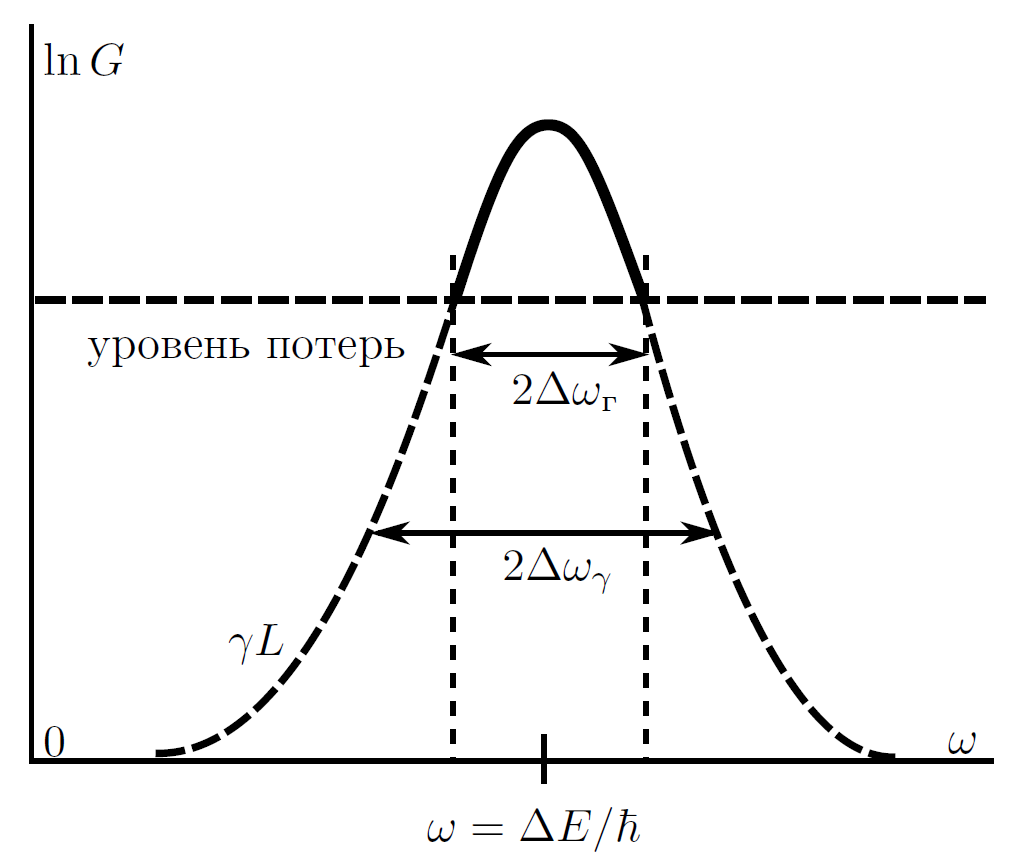
\includegraphics[width=0.38\textwidth]{../Изображения/Порог генерации.png}
\end{wrapfigure}

Пусть зеркала имеют коэффициенты отражения $r_1$ и $r_2$. Дополнительные потери 
энергии в одном проходе равны $T$, тогда условие достижения порога генерации 
определяется выражением:
\begin{equation}
	G r_1 r_2 T \ge 1 \Leftrightarrow 2 \gamma L \ge - \ln T - \ln r_1 r_2
	\label{eq:G}
\end{equation}
Генерация может происходить только в том диапазоне частот $\omega \pm \Delta 
\omega_г$, в котором справедливо полученное соотношение.

В лазерах с непрерывной генерацией в установившемся режиме $G = \frac{1}{T r_1 
r_2}$, но чтобы лазер имел ненулевую выходную мощность коэффициент $G$ 
активного материала в отсутствии обратной связи должен быть больше порогового 
значения (\ref{eq:G}).

\subsection*{Накачка энергии}

Покажем, что состояние активного вещества, при котором $N_1 > N_0$ 
термодинамически неравновесно. Согласно распределению Больцмана 
$\frac{N_1}{N_0} = \exp \left(- \frac{E_1 - E_0}{k T}\right)$, если $N_1 > 
N_0$, то $T < 0$. Поэтому, чтобы активное вещество имело инверсную заселённость 
необходимо, чтобы система была не замкнута и имелась постоянная подкачка 
энергии из внешних источников.

\begin{wrapfigure}{l}{0.2 \textwidth}
	\centering
	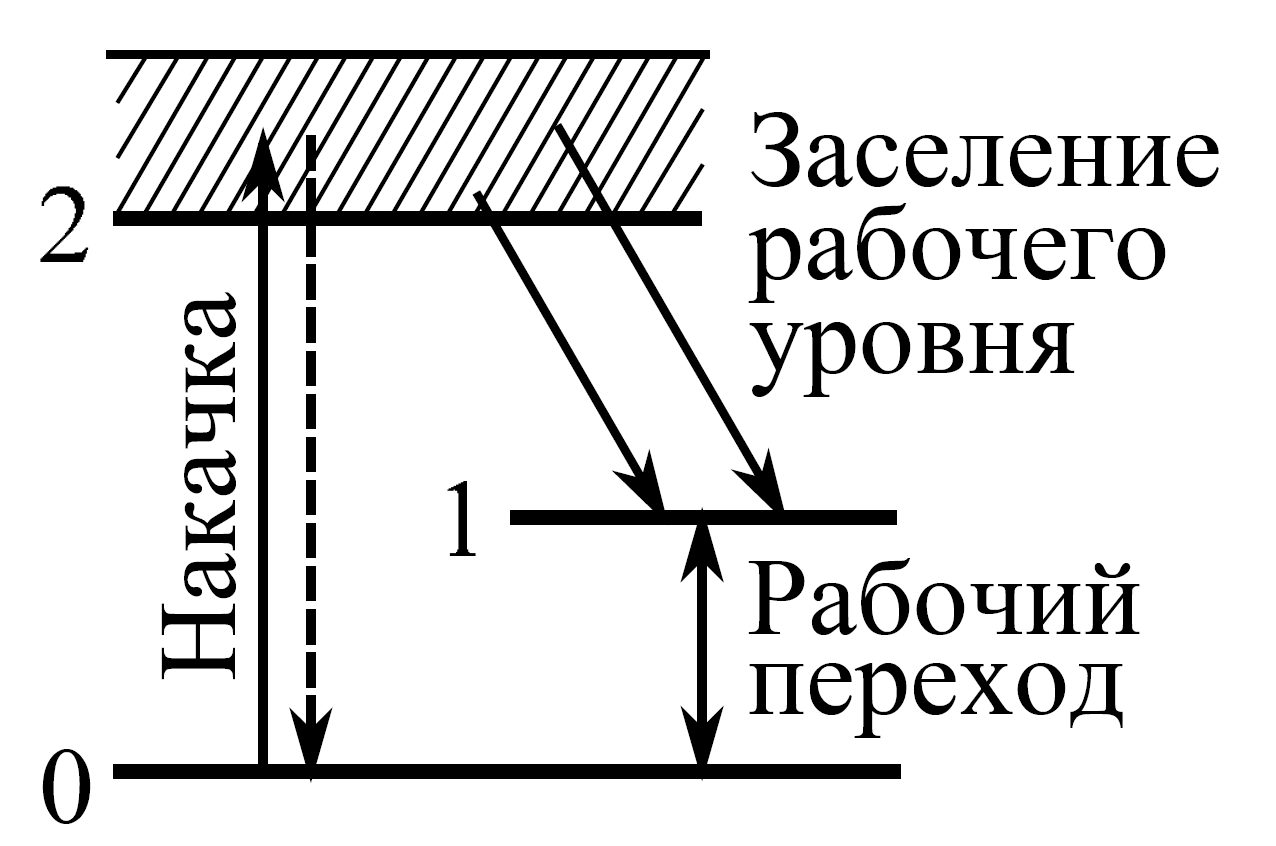
\includegraphics[width=0.18\textwidth]{../Изображения/Накачка.png}
\end{wrapfigure}

Рассмотрим метод оптической накачки энергии. Активное вещество облучается 
электромагнитной волной такой частоты, что атомы среды переходят в возбуждённое 
состояние. Так как вероятность поглощения и вынужденного излучения фотона 
равны, то для двухуровненой энергетической системы оптическая накачка не 
возможна. Поэтому используются трёх- или четёрыхуровненые системы.

С помощью накачки атомы переводятся из основного состояния 0 в возбуждённое 2. 
Из состояние 2 атомы могут перейти либо в состояние 0, либо в состояние 1. В 
состоянии 1 атомы будут накапливаться, если время нахождения атома в этом 
состоянии было достаточно велико. Это время можно оценить из соотношения 
неопределённостей $\Delta E \tau \sim \hslash$, поэтому 1 уровень обладает 
узкой энергетической полосой $\Delta E$. Уровень 2 стараются выбрать широким, 
чтобы накачка энергии происходила наиболее эффективно -- была задействована 
большая часть спектра электромагнитной волны накачки.

\subsection*{Продольные моды лазерного излучения}

Рассмотрим продольные моды в резонаторе Фабри-Перо с активным веществом 
заполняющим всё пространство резонатора и имеющим показатель преломления $n = 
1$, расстояние между зеркалами $L$.

Волна должна распространяться строго перпендикулярно зеркалам, иначе она через 
какое-то время покинет резонатор и не будет достаточно усилена. Тогда в 
резонаторе будут наблюдаться стоячие волны $E \propto \sin(\omega t) \sin 
(kx)$, если зеркала проводящие, то на длине резонатора должно укладываться 
целое число полуволн:
$$
k_q L = \pi q
$$
где $q \in \mathbb{N}$ -- номер моды, $k_q = \frac{\omega_q}{c}$ -- волновое 
число. Из полученного соотношения определим допустимые собственные частоты 
резонатора:
$$
\omega_q = q \frac{\pi c}{L}
$$
Таким образом, спектром генерации лазерного излучения является набор $\omega_q 
\pm \Delta \Omega$ узких спектральных линий.

%\subsection*{2.2. Спектр лазерного излучения}
% Две картинки добавить.
%\subsection*{Когерентность лазерного излучения}
